\documentclass[10pt,a4paper]{article}
\usepackage{arabtex}
\usepackage[OT1,T1,LFE,LAE]{fontenc}
\usepackage[utf8]{inputenc}
\usepackage[arabic,english,farsi]{babel}
\usepackage{amsmath,amsfonts} % Math packages
\usepackage{amssymb}
%\usepackage{cmap}

\usepackage{multicol}

\usepackage{graphicx}
\usepackage[caption=false]{subfig}
\usepackage{color}
\usepackage{float}
\usepackage{sidecap}
%\sidecaptionvpos{figure}{c}
\usepackage{anysize}
\marginsize{2cm}{2cm}{2cm}{2cm}

\usepackage{listings}

\usepackage{appendix}
%\renewcommand{\appendixname}{Apéndices}
%\renewcommand{\appendixtocname}{Apéndices}
%\renewcommand{\appendixpagename}{Apéndices}

\usepackage[colorlinks=true,plainpages=true,citecolor=blue,linkcolor=blue,urlcolor=cyan]{hyperref}
%\usepackage{hyperref}


%%% Equation and float numbering
\numberwithin{equation}{section}
\numberwithin{figure}{section}
\numberwithin{table}{section}


\newcommand{\horrule}[1]{\rule{\linewidth}{#1}}    % Horizontal rule

\newcommand{\titleText}{Bridges, LANs and the Cisco IOS \\ Laboratory Manual}

\title{
\normalsize In the name of Allah\\
\vspace{10pt}
\LARGE\FR{بسم \allah\  الرحمن الرحیم}
\vspace{10pt}
\begin{center}
    %	\newcommand{\HRule}{\rule{\linewidth}{0.5mm}}
    \begin{minipage}{0.48\textwidth}
        \begin{flushleft}
            
\includegraphics[height=64pt,width=64pt]{../img/logo.png}
        \end{flushleft}
    \end{minipage}
    \begin{minipage}{0.48\textwidth}
        \begin{flushright}
            
\includegraphics[height=64pt]{../img/eng-logo.png}
        \end{flushright}
    \end{minipage}
\end{center}
\vspace*{-64pt}
%	\horrule{0.5pt} \\[0.4cm]
\huge \titleText\\
\vspace{40pt}
%	\horrule{2pt} \\[0.5cm]
}
\author{
\huge University of Tehran\\
\LARGE \FR{دانشگاه تهران}\\
\\
\LARGE School of Electrical and Computer Engineering\\
\FR{دانشکده مهندسی برق و کامپیوتر}\\
\\
\Large Computer Network Lab\\
\FR{آزمایشگاه شبکه‌های کامپیوتری}\\
\\
\\
\\
\normalfont
Dr. Ahmad Khonsari - \FR{احمد خونساری}\\
\href{mailto:a_khonsari@ut.ac.ir}{a\_khonsari@ut.ac.ir}\\
\\
\normalsize
Amir Haji Ali Khamseh'i - \FR{امیر حاجی علی خمسه‌ء}\\
\href{mailto:khamse@ut.ac.ir}{khamse@ut.ac.ir}\\
\\
\normalsize \href{mailto:m.borhani@ut.ac.ir}{Muhammad Borhani} - \FR{محمد برهانی}\\
\normalsize \href{mailto:a.a.khordadi@ut.ac.ir}{Amirahmad Khordadi} - \FR{امیراحمد خردادی}\\
\normalsize \href{mailto:sina\_kashipazha@ut.ac.ir}{Sina Kashi pazha} - \FR{سینا کاشی پزها}\\
\normalsize \href{mailto:mashahsavand@ut.ac.ir}{Mohammad Ali Shahsavand} - \FR{محمد علی شاهسوند}
}

\date{\vspace{30pt}\today\\\vspace{10pt}{\selectlanguage{farsi}\today}}

\usepackage{fancyhdr}
\pagestyle{fancy}
%\pagestyle{fancyplain}
\fancyhf{}
\fancyhead[L]{\footnotesize Computer Network Lab \\ \FR{آزمایشگاه شبکه‌های کامپیوتری}}
\fancyhead[R]{\footnotesize \titleText}
\fancyfoot[R]{\footnotesize School of Electrical and Computer Engineering\\\FR{دانشکده مهندسی برق و کامپیوتر}}
\fancyfoot[C]{\thepage}
\fancyfoot[L]{\footnotesize University of Tehran \\ \FR{دانشگاه تهران}}
\renewcommand{\footrulewidth}{0.8pt}
\renewcommand{\headrulewidth}{1pt}            % Remove header underlines
\renewcommand{\footrulewidth}{1pt}                % Remove footer underlines
\setlength{\headheight}{13.6pt}

\usepackage{tikz}
\usetikzlibrary{calc}

\begin{document}
    \selectlanguage{english}

    %\vspace*{-1.5cm}
    \maketitle

    %\tableofcontents

    \pagebreak
    %Arabic \AR{\allah}
    %Persian \FR{فروشگاه}
    %Arabic \foreignlanguage{arabic}{كحض}
    %Persian \foreignlanguage{farsi}{فروشگاه}



    %	يعود تاريخ علوم الحاسوب إلى
    %\chapter
    %\section
    %\subsubsection
    %\subsection
    %\section
    %\chapter
    %\part
    %\caption
    %\end{otherlanguage}


    \section*{Exercises on Cisco IOS}
    The students in the lab should divide themselves into four groups for the first four exercises. Each group uses two workstations, a bridge, and two hubs, which are required to be connected as shown in Fig. 3.7, Table 3.2 and Table 3.3.

    \section{ Exercise 1}
    In this exercise we build the connection to the router. \\
    Identify the cable from your workstation and the cable from your router interface (see Fig. 3.7, Table 3.2 and Table 3.3).
    Plug these two cables into your hub.
    In this case, you have built a LAN segment with a \textit{star} topology.
    Your partner should build a star LAN segment on the other side of the router. \\
    \begin{figure}[H]
        \centering
        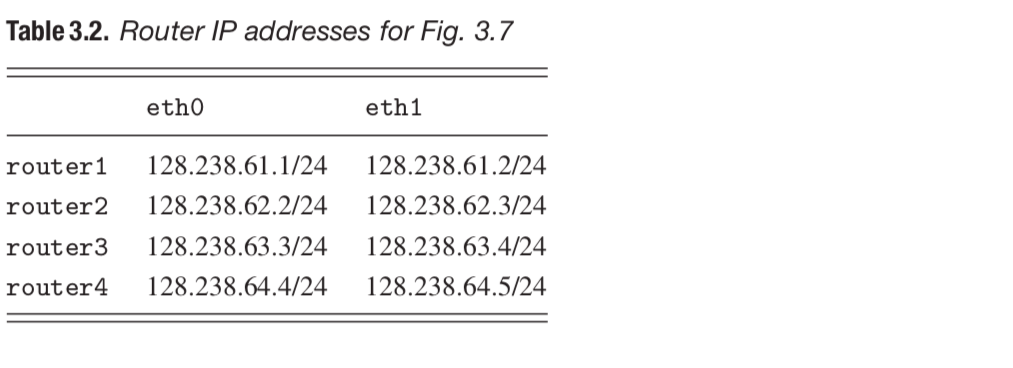
\includegraphics[width=0.9\textwidth]{img/table3-2.png}
    \end{figure}
    \begin{figure}[H]
        \centering
        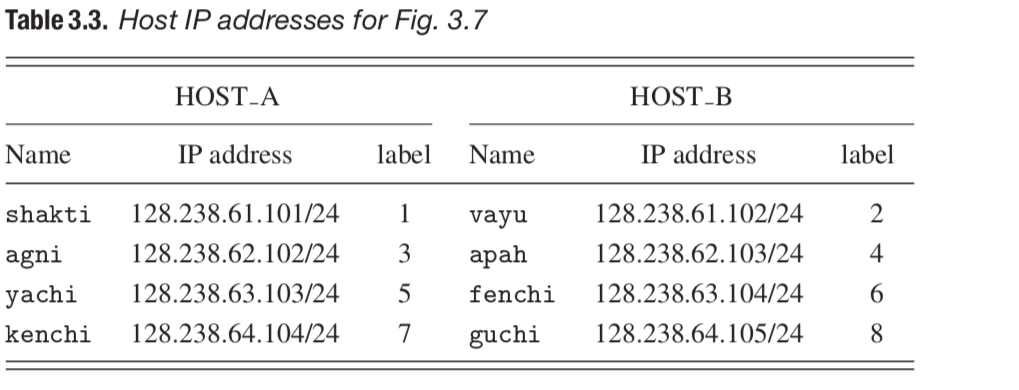
\includegraphics[width=0.9\textwidth]{img/table3-3.png}
    \end{figure}
    \begin{figure}[H]
        \centering
        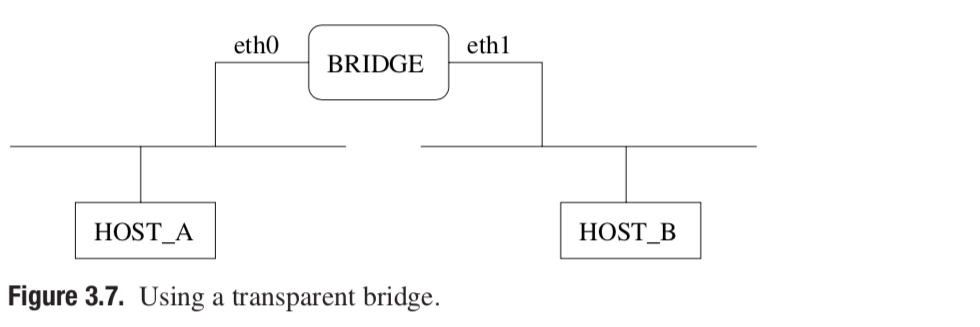
\includegraphics[width=0.9\textwidth]{img/figure3-7.png}
    \end{figure}
    After running \textbf{tcpdump -enx} on both workstations, turn on the router. Capture the
    gratuitous ARP sent by the router. \\
    Change the IP address of your workstation to be in the same subnet as the router.
    You can choose any valid host id for your host. \\
    \textbf{ping} the router interface to test the connection to the router.
    \subsection*{Report}
    Submit the gratuitous ARP sent by the router. What is the default IP address of the router interface? \\


    \section{ Exercise 2}
    Telnet to your router. When prompted for a login password, type \texttt{el537}.
    You should now be in the \textit{User EXEC} mode. \\
    Type \textbf{help} to learn how to use the online help.
    Study Fig. 3.6. Navigate through the \textit{User EXEC}, \textit{Privileged EXEC}, \textit{Global Configuration}, and \textit{Interface Configuration} modes. In each mode, type \textbf{?} to display a list of available commands and study these commands. \\
    Type \textbf{show version} in the \textit{User EXEC} mode to display the Cisco IOS banner.
    Identify which Cisco IOS Release is running in the router.
    Save the Cisco IOS banner for your lab report.
    \subsection*{Report}
    Submit the Cisco IOS banner you saved.
    Identify the release of the Cisco IOS software in the router.

    \section*{A simple bridge experiment}
    Figure 3.7 shows a simple case of the use of bridges, which consists of two network segments connected by a bridge.
    With this simple topology, we can easily capture initial BPDUs before each bridge is engaged in the spanning tree calculation. \\
    Configure transparent bridging as in Fig.
    3.7, Table 3.2 and Table 3.3.
    Note that the default configuration of the hosts and the bridges are different from those in the tables.
    You need to change the IP addresses of the bridge interfaces,\footnote{As soon as you change the IP address of the bridge interface your host is connected to, the \textbf{telnet} connection will be lost.
    You need to again change the IP address of your workstation to be in the same subnet as the bridge interface. See Section 3.3.3.} as well as set the bridge group and enable the spanning tree algorithm (see the previous section on bridge configuration).
    Do the following experiments.

    \section{ Exercise 3}
    Configure the IP addresses of your workstation and the bridge interfaces as shown in Fig. 3.7, Table 3.2 and Table 3.3.
    To avoid confusion, each bridge should be configured by only one person. \\
    Run \textbf{tcpdump -en ip proto 1} on your machine, and your partner’s machine. Send \textbf{ping} messages to your partner’s machine: \textbf{ping -sv} \textit{remote-machine}.
    After receiving the tenth echo reply, quit the \textbf{ping} process, and save the \textbf{tcpdump} outputs from both machines. \\
    During this exercise, don’t run \textbf{ping} programs at the same time. For clean results, do your experiments in turn.
    \subsection*{Report}
    What are the IP and MAC addresses of a packet that went from your machine to the bridge?
    What are the IP and MAC addresses of a packet that went from the router to your partner’s machine? \\
    Answer the same questions, but for the echo reply that was returned from your partner’s machine. \\
    Using the \textbf{tcpdump} outputs from both machines, calculate the average delay that a packet experienced in the bridge.
    Note that the system times of the two machines might be different.
    Show all the steps and submit the \textbf{tcpdump} outputs with your report.


    \section{ Exercise 4}
    Run \textbf{tcpdump -e -c 5 ether multicast} on your workstation to capture 5 BPDUs messages generated by the bridge.
    Save the BPDUs for the lab report. \\
    You need to collect all the different BPDUs from other students in your lab.
    At this time, however, just save your BPDU in the \texttt{guest} home directory (which is \texttt{/home/guest/})as \textit{“name of your host.ex4”} since there is no network connections to hosts in the other groups.
    In our next exercise, after we put all the workstations in one network as shown in Fig. 3.8, you can collect BPDUs from other workstations using \textbf{ftp}. \\
    You should collect eight different BPDUs in this exercise.
    These BPDUs will be helpful when studying the spanning tree algorithm later in this chapter.

    \subsection*{Report}
    How frequently (in seconds) does a bridge sends its BPDUs? \\
    Submit the eight different BPDUs you saved.
    Identify the values of root ID, root path cost, bridge ID, and port ID for each BPDU\footnote{You may ask the lab instructor for the physical addresses of network interfaces, and record them in Table A.1 and Table A.2. You need the MAC addresses to help analyze the BPDUs.}.

    \section*{Spanning tree exercises}
    In this section, we will use Fig. 3.8 as our network topology.
    You need to change the IP addresses of the bridge interfaces, as well as that of your workstation. Refer to Section 3.3.4 on how to configure a transparent bridge.
    Also see Section 3.3.3 on how to handle a frozen telnet session after you change the bridge IP address. \\
    Upon being started, a transparent bridge learns the network topology by analyzing source addresses of incoming frames from all attached networks.
    The next exercise shows the process by which a transparent bridge builds its filtering database.
    \begin{figure}[H]
        \centering
        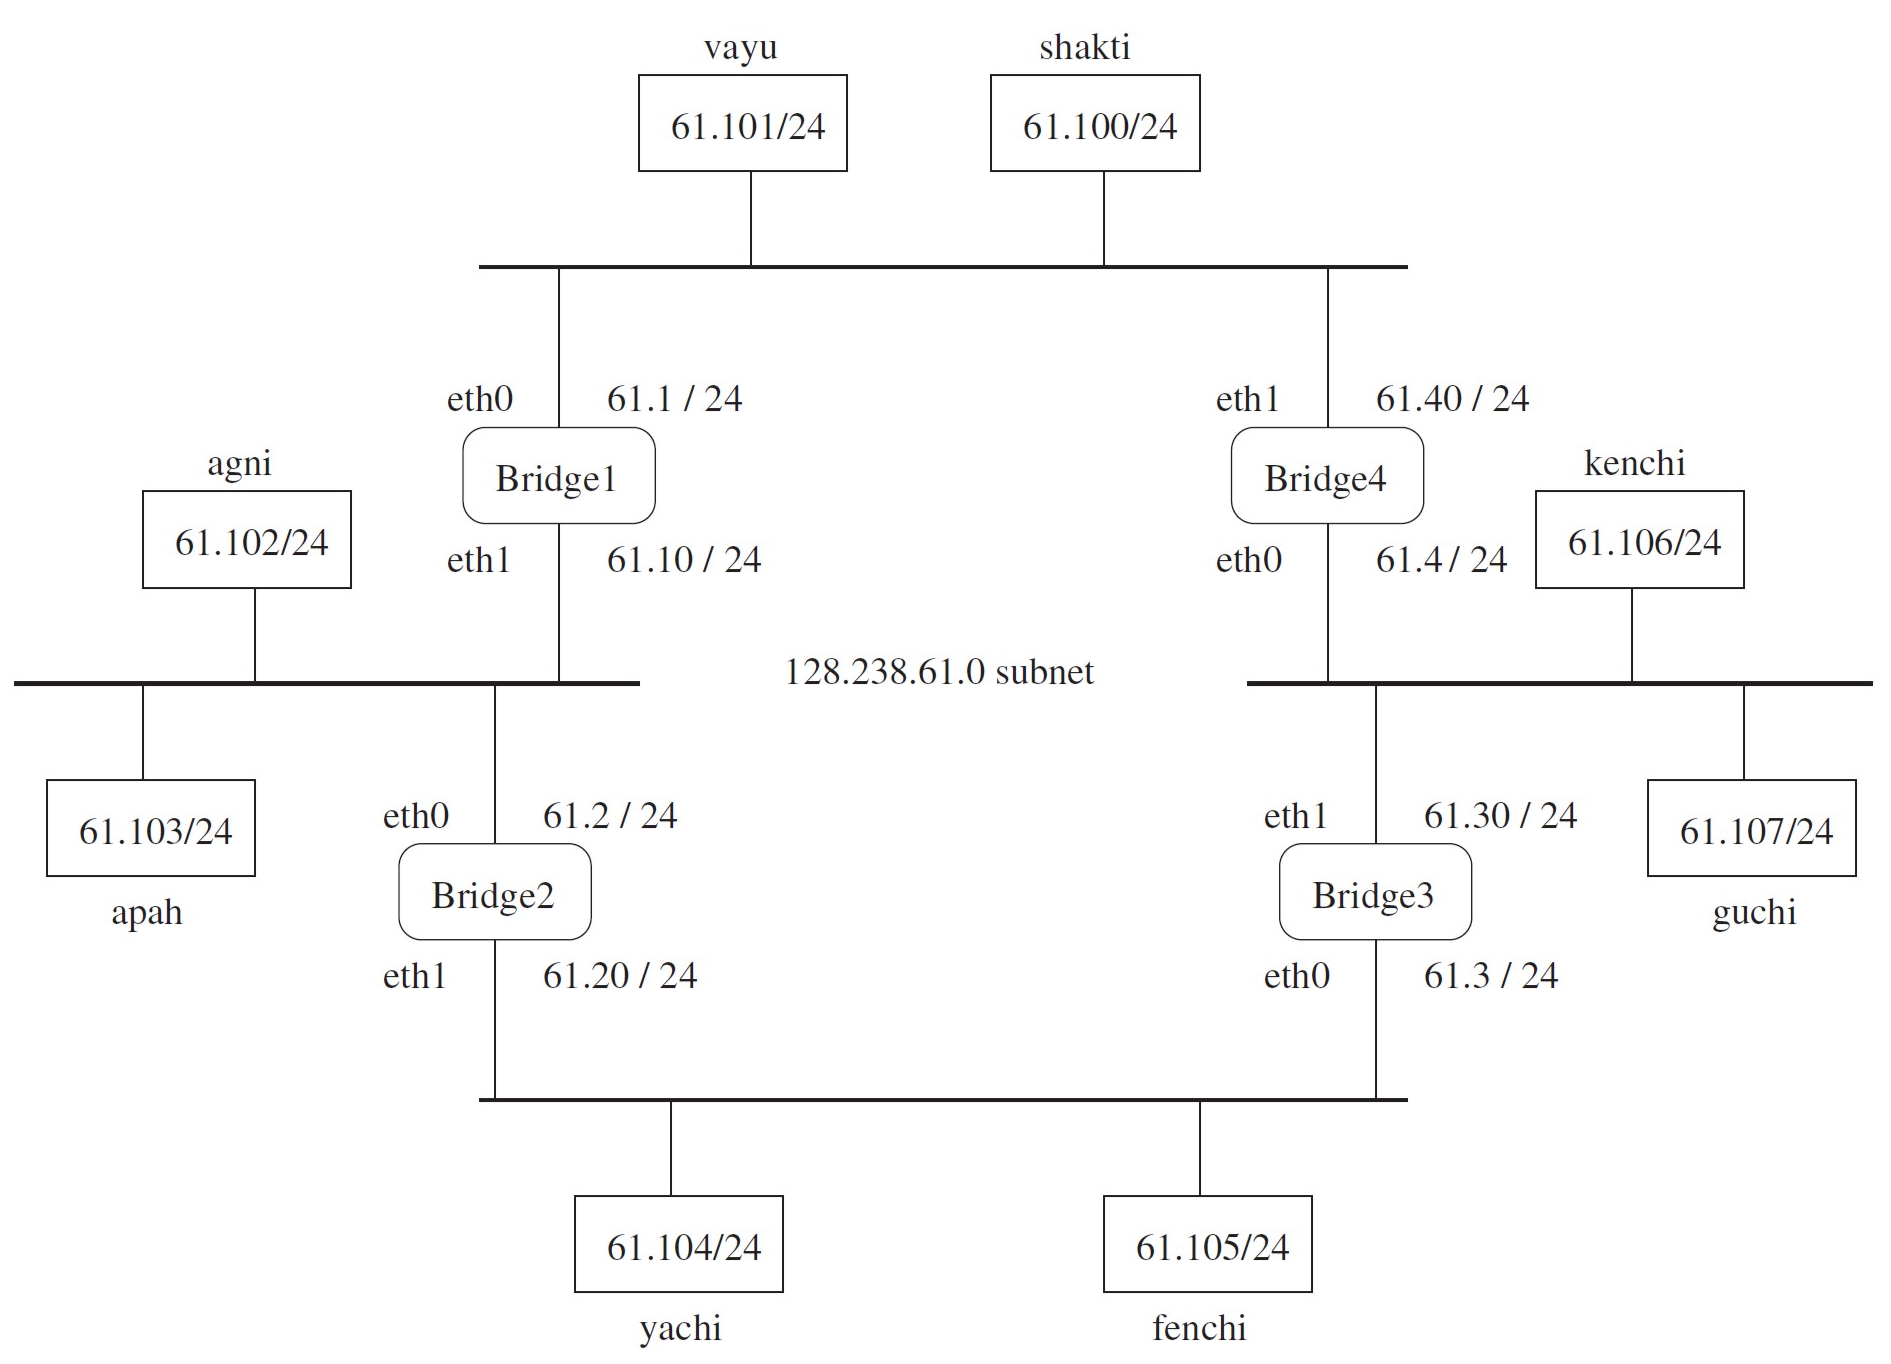
\includegraphics[width=0.9\textwidth]{img/figure3-8.png}
    \end{figure}

    \section{ Exercise 5}
    After configuring the network in Fig. 3.8, login to the bridge. \\
    Get to the \textit{Privileged EXEC} mode. Type \textbf{show bridge} to see the entries in the bridge forwarding database. \\
    Whenever you \textbf{ping} or \textbf{telnet} from your workstation to a host that is not in the table, observe how the filtering database in the bridge is expanded. \\
    You may use the \textbf{clear bridge} \textit{group} command to remove any learned entries from the filtering database, if you see a full filtering database or if you want to repeat the above exercise. \\
    \subsection*{Report}
    From the output of \textbf{show bridge}, identify which bridge ports are blocked, and which ports are in the forwarding state for each bridge.

    \section{ Exercise 6}
    Using \textbf{tcpdump -ex ether multicast}, capture the BPDU packet flowing on your network segment. \\
    \textbf{Telnet} to the hosts in the other three LAN segments and execute the above \textbf{tcpdump} command in the \textbf{telnet} window to collect BPDUs sent there. \\
    Login to each bridge to collect the \textbf{show bridge} outputs.
    \subsection*{Report}
    Submit the four different BPDUs you saved.
    Identify the values of root ID, root path cost, bridge ID, and port ID for each BPDU. \\
    Based upon the initial BPDUs saved in Exercise 4, draw the spanning tree seen by the BPDUs. Identify the root ports and the root path cost (in hop counts) for each bridge.
    Identify the designated bridge and the designated port for each LAN segment.
    Identify the state of each bridge port (blocking or forwarding). \\
    Don’t just assume that \texttt{Bridge1} has the highest priority for the root bridge.
    Draw the spanning tree based upon your data (eight initial BPDUs). \\
    Write the final BPDUs you collected using the three-tuple format: \textit{{root ID, root path cost, bridge ID}}. \\
    Once you have the spanning tree, justify it using the four final BPDUs collected in this exercise and/or the output of the \textbf{show bridge} command. \\
    \section{ Exercise 7}
    This exercise is performed by all the students together.
    First, send \textbf{ping} messages from \texttt{apah} to \texttt{yachi}, while \textbf{tcpdump} is running.
    Let the two programs run during this exercise. \\
    Then, disconnect the cable from the \texttt{ethernet0} port of \texttt{Bridge2} from the hub, and type the \textbf{time} command on \texttt{apah} or \texttt{yachi} to get the current time. \\
    Observe the \textbf{ping} and \textbf{tcpdump} windows. When the connection is reestablished, type the \textbf{time} command again. How long does it take the spanning tree algorithm to react to the change in the topology? \\
    Once you can successfully reach other hosts, get to the bridges to run \textbf{show bridge} to collect the port states. Also collect BPDUs from all the LAN segments as you did in the previous exercise. \\
    After every student has collected the required data, connect the cable to the original position. Again, measure the time it takes for the bridges to adapt to the new change.
    \subsection*{Report}
    Draw the new tree formed after the cable was disconnected, based on the BPDUs you collected in this exercise. Specify the state of each bridge port.


    \section*{Exercise on the Cisco IOS web browser UI}
    \section{ Exercise 8}
    You can also configure a router using the web browser UI. To enable the web server, login to the router and execute \textbf{ip http server} in the \textit{Global Configuration} mode. \\
    Next, start a web browser (e.g., \texttt{Mozilla} in Linux, or \texttt{Hotjava} in Solaris) in your host, and enter the IP address of the router interface. When prompted, enter \texttt{el537} for password, and leave the \texttt{User Name} field blank. Then you can browse the router configuration web pages and configure the router there.

\end{document}











